\newpage
\onecolumngrid
\section{Parameter file}
A snippet of an INGRID parameter file is shown below. Extensive documentation and tutorials for parameter file setup can be found in the INGRID Read The Docs documentation online.
\begin{lstlisting}[basicstyle=\small, aboveskip=\bigskipamount, frame=single, captionpos=b, caption={Snippet of YAML formatted configuration file. YAML files utilize Python formatted comments, keyword-value mappings, and nesting of structures via indentation.}]
# ---------------------------------------------------
# User data directories
# ---------------------------------------------------
dir_settings:
  eqdsk: ../data/SNL/DIII-D/  # dir containing eqdsk
  limiter: .  # dir containing limiter
  patch_data: ../data/SNL/DIII-D/  # dir containing patch data
  target_plates: ../data/SNL/DIII-D/ # dir containing target plates
# ---------------------------------------------------
# eqdsk file name
# ---------------------------------------------------
eqdsk: neqdsk
# ---------------------------------------------------
# General grid settings
# ---------------------------------------------------
grid_settings:
  # ----------------------------------------------------------------------------
  # Settings for grid generation (num cells, transforms, distortion_correction)
  # ----------------------------------------------------------------------------
  grid_generation:
    distortion_correction:
      all:
        active: True # true, 1 also valid.
        resolution: 1000
        theta_max: 120.0
        theta_min: 80.0
    np_default: 3
    nr_default: 3
    poloidal_f_default: x, x
    radial_f_default: x, x
  # ---------------------------------------------------
  # guard cell size
  # ---------------------------------------------------
  guard_cell_eps: 0.001
  # ---------------------------------------------------
  # num levels in efit plot
  # ---------------------------------------------------
  nlevs: 30
  # ---------------------------------------------------
  # num xpts
  # ---------------------------------------------------
  num_xpt: 1
  patch_generation:
    strike_pt_loc: target_plates # 'limiter' or 'target_plates'
    rmagx_shift: 0.0
    zmagx_shift: 0.0
  # ---------------------------------------------------
  # Psi levels
  # ---------------------------------------------------
  psi_1: 1.066
  psi_core: 0.95
  psi_pf_1: 0.975
  # ---------------------------------------------------
  # magx coordinates
  # ---------------------------------------------------
  rmagx: 1.75785604
  zmagx: -0.0292478683
  # ---------------------------------------------------
  # xpt coordinates
  # ---------------------------------------------------
  rxpt: 1.300094032687
  zxpt: -1.133159375302
  # ---------------------------------------------------
  # Filled contours vs contour lines
  # ---------------------------------------------------
  view_mode: filled
# ---------------------------------------------------
# Saved patch settings
# ---------------------------------------------------
patch_data:
  file: LSN_patches_1597099640.npy
  preferences:
    new_file: true
    new_fname: LSN_patches_1597099640.npy
  use_file: false
# ---------------------------------------------------
# Integrator
# ---------------------------------------------------
integrator_settings:
  dt: 0.01
  eps: 5.0e-06
  first_step: 5.0e-05
  max_step: 0.064
  step_ratio: 0.02
  tol: 0.005
# ---------------------------------------------------
# Limiter settings
# ---------------------------------------------------
limiter:
  file: ''
  use_efit_bounds: false
# ---------------------------------------------------
# target plate settings
# ---------------------------------------------------
target_plates:
  plate_E1:
    file: d3d_otp.txt
    zshift: -1.6
  plate_W1:
    file: d3d_itp.txt
    zshift: -1.6
\end{lstlisting}

\newpage
\section{TCV SF-75 comparison of grids and UEDGE simulation results}
We include figures illustrating consistent results between INGRID and UEDGE grid generators. These grids were then utilized to for UEDGE simulations.
\begin{figure}[H]
    \centering
        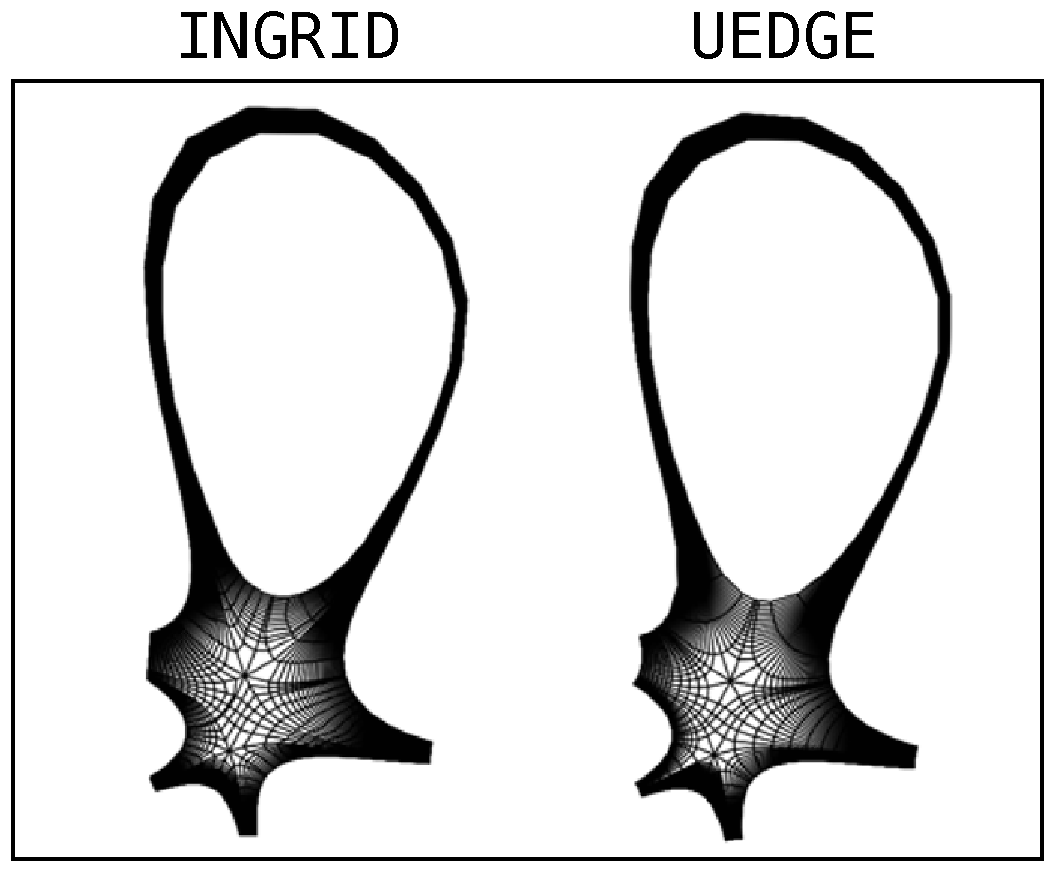
\includegraphics[width=0.9\textwidth]{figures/benchmark/gridue_both.pdf}
        \caption{INGRID and UEDGE generated TCV SF-75 grids.}
        \label{fig:ingrid_grid}
\end{figure}
\begin{figure}[H]
    \centering
        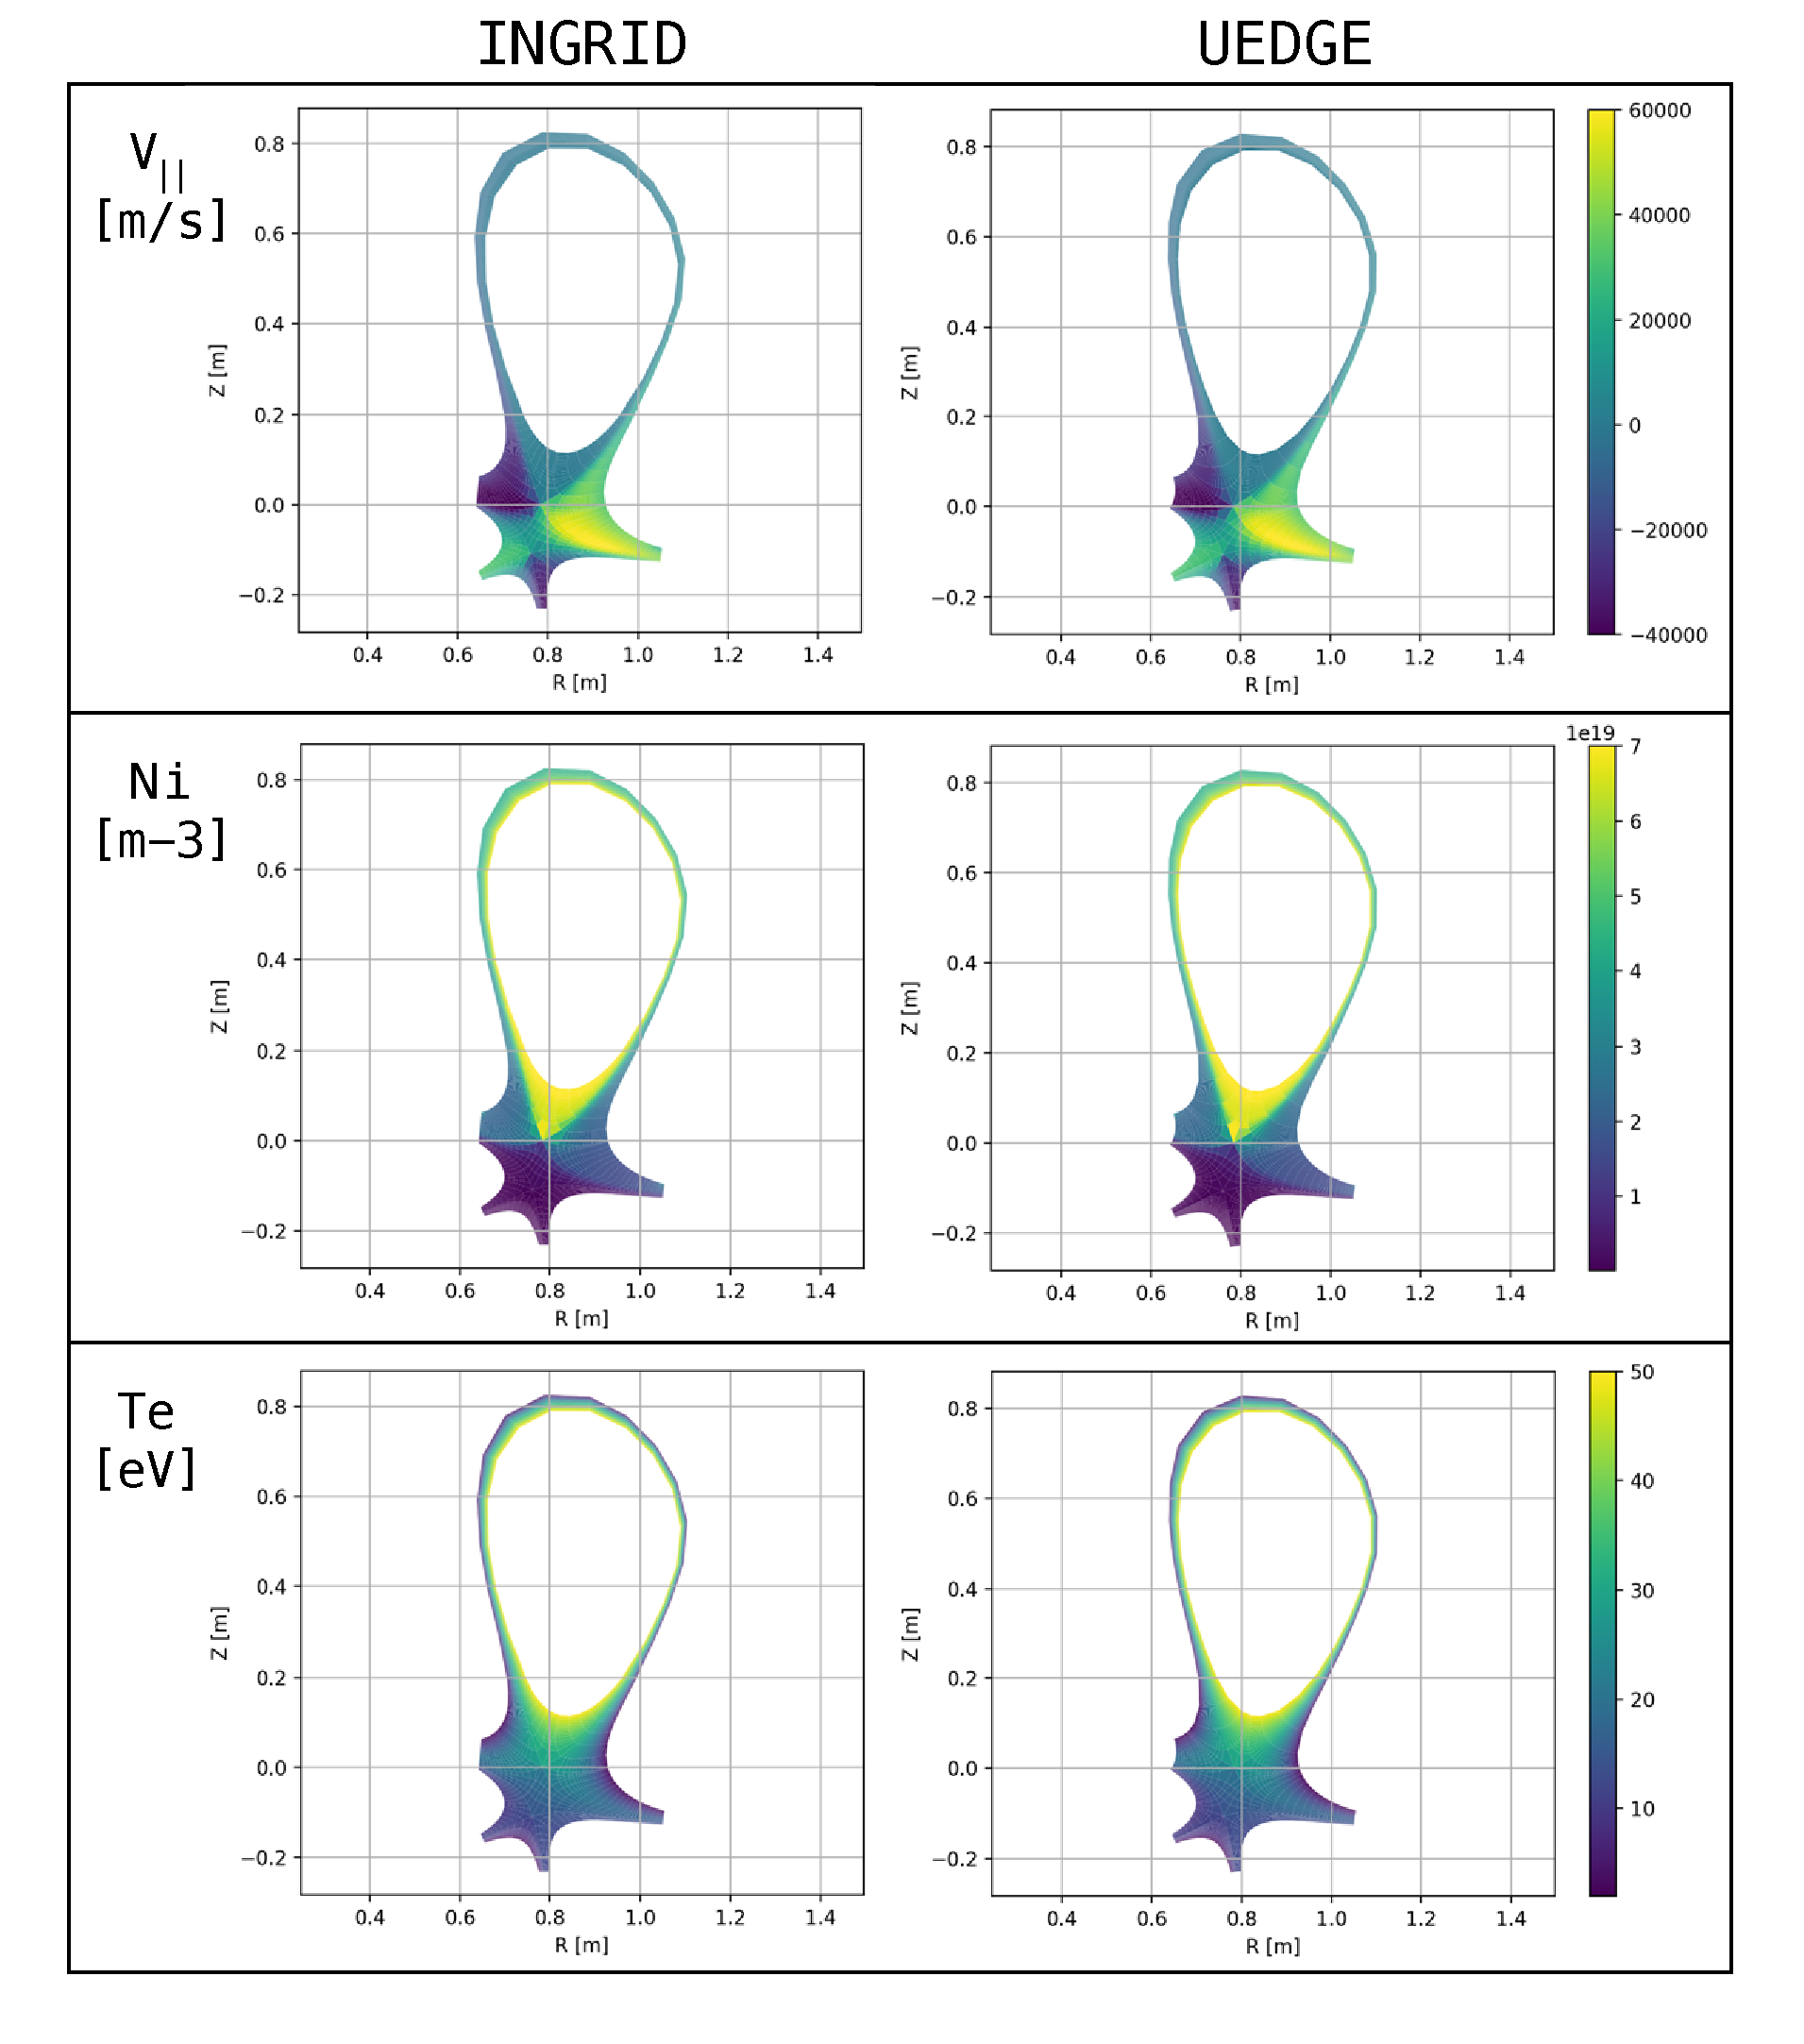
\includegraphics[width=\textwidth]{figures/benchmark/BenchmarkCollection.pdf}
        \caption{A collection of UEDGE simulations run on INGRID and UEDGE generated grids.}
        \label{fig:benchmark_collection}
\end{figure}

\section{Supported divertor configurations}
\begin{figure}[H]
    \centering
        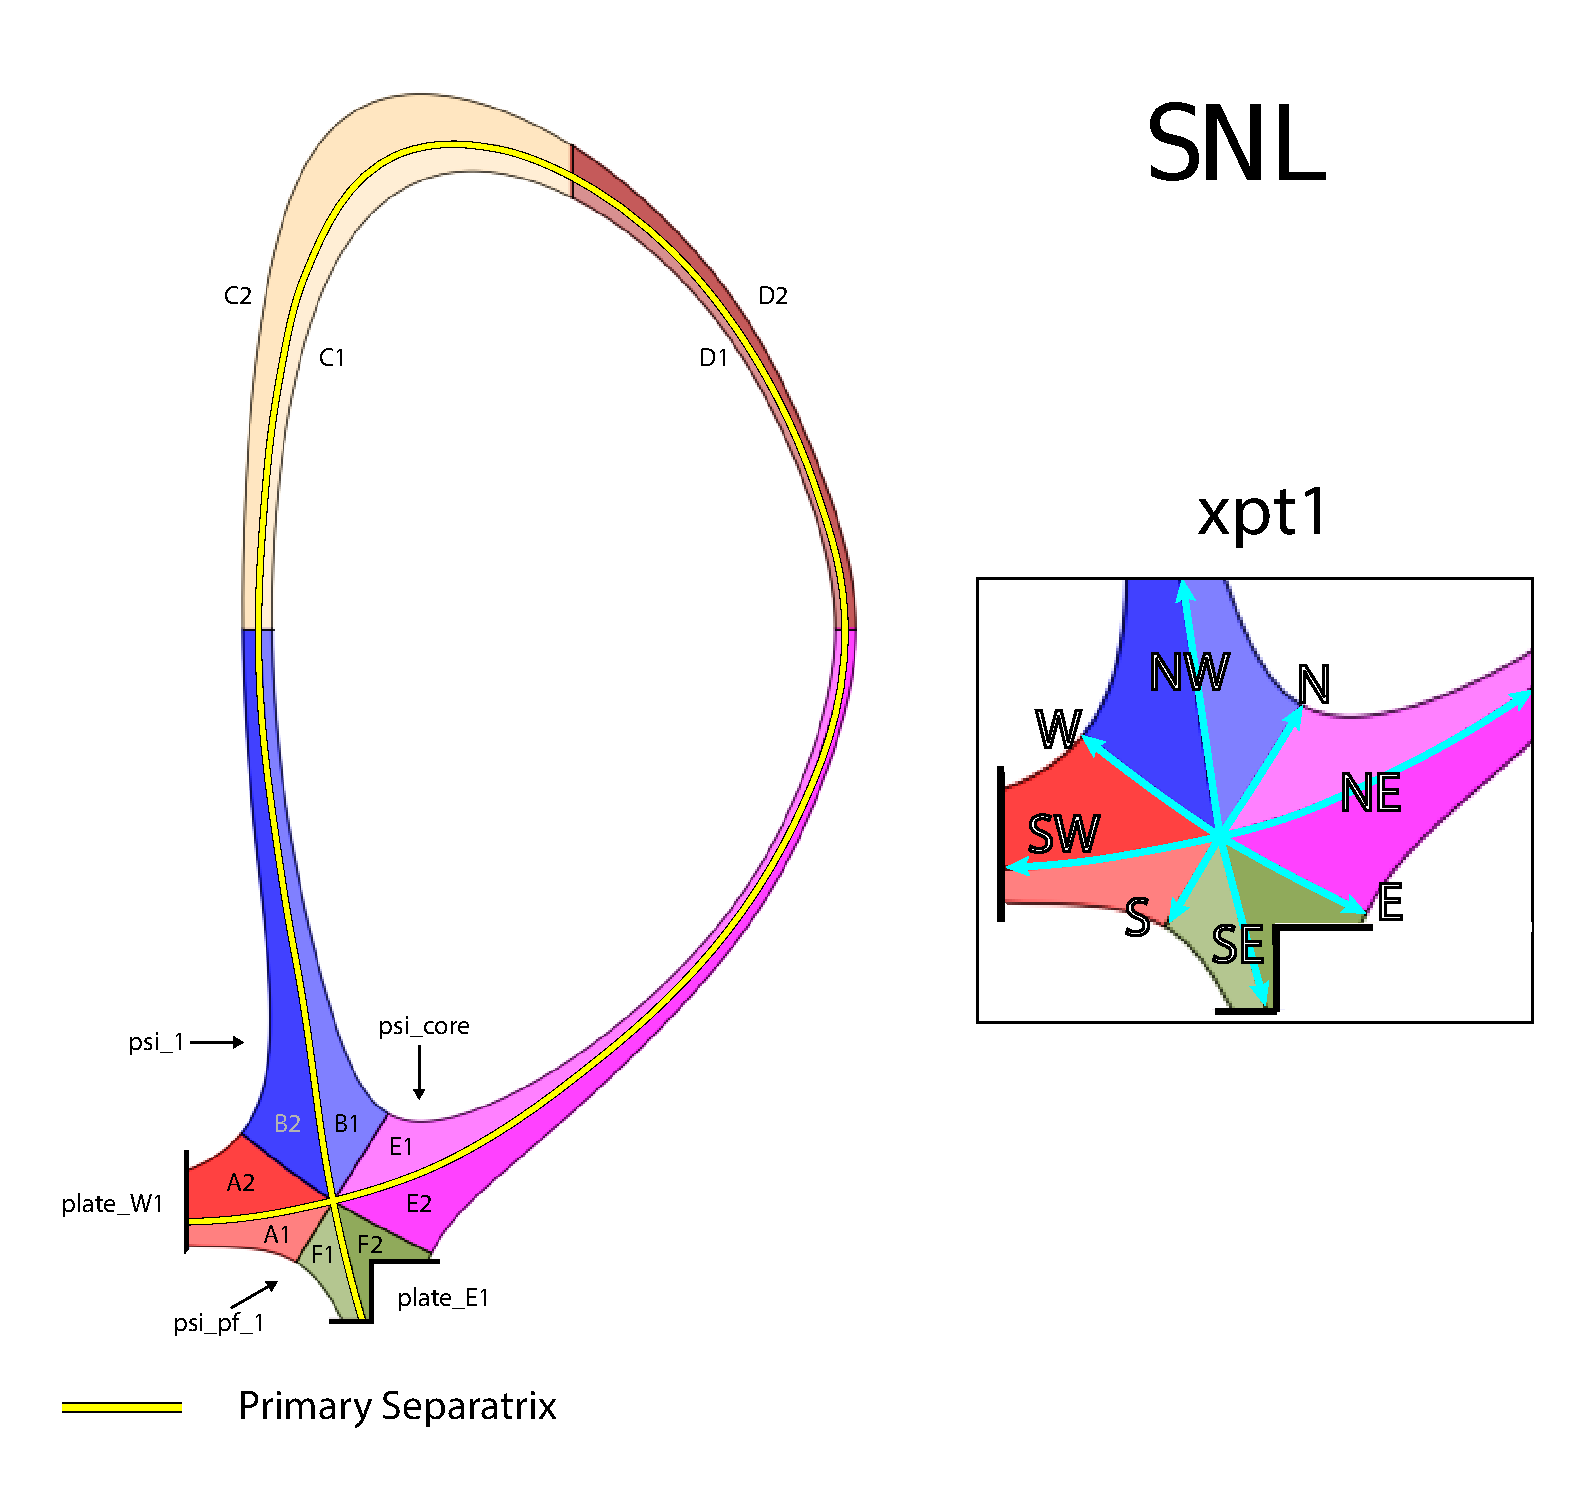
\includegraphics[width=\textwidth]{figures/configurations/SNL_collection.pdf}
        \caption{SNL Patch map}
        \label{fig:snl_patch_map}
\end{figure}
\begin{figure}[H]
    \centering
        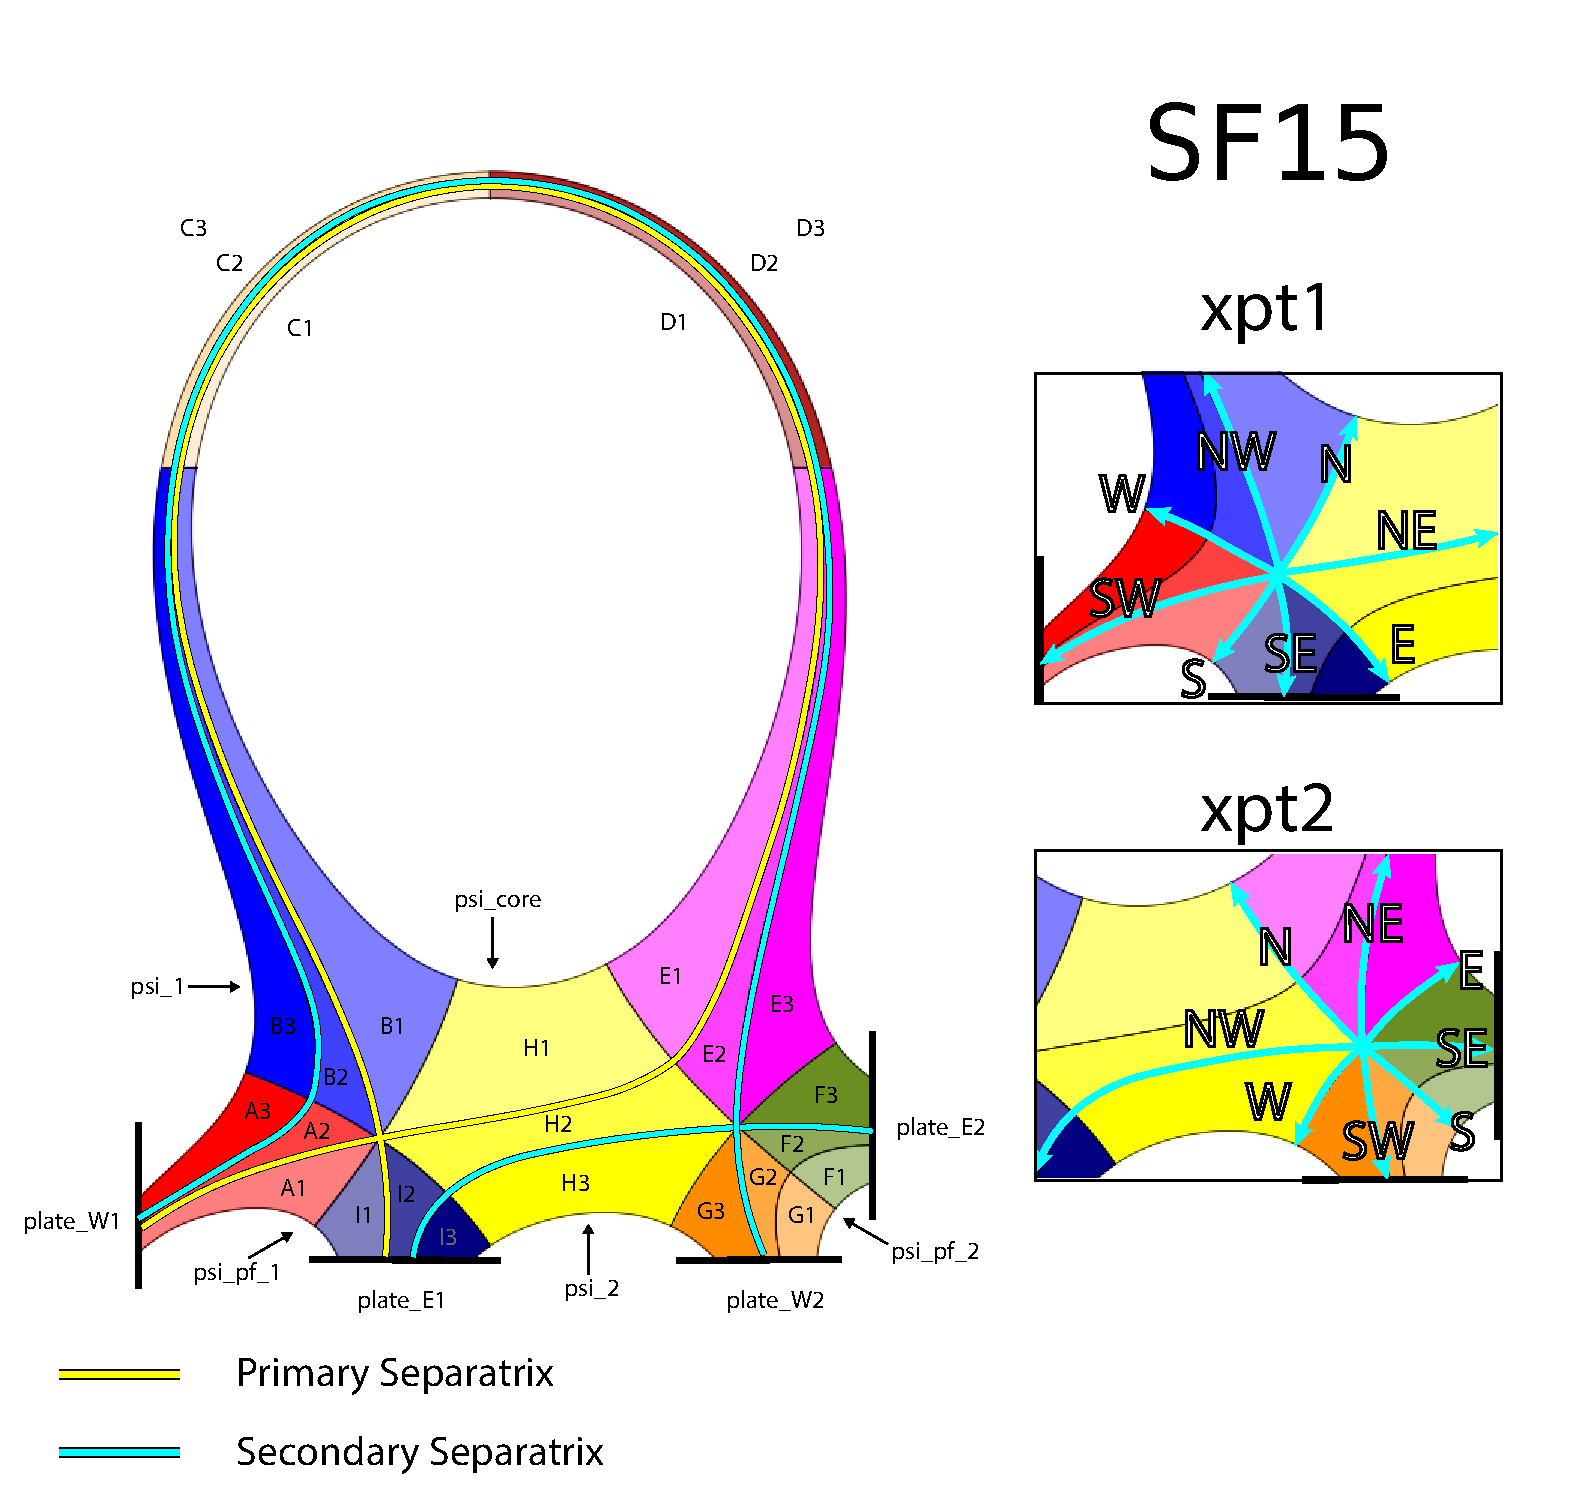
\includegraphics[width=\textwidth]{figures/configurations/SF15_collection.pdf}
        \caption{SF15 Patch map}
        \label{fig:sf15_patch_map}
\end{figure}
\begin{figure}[H]
    \centering
        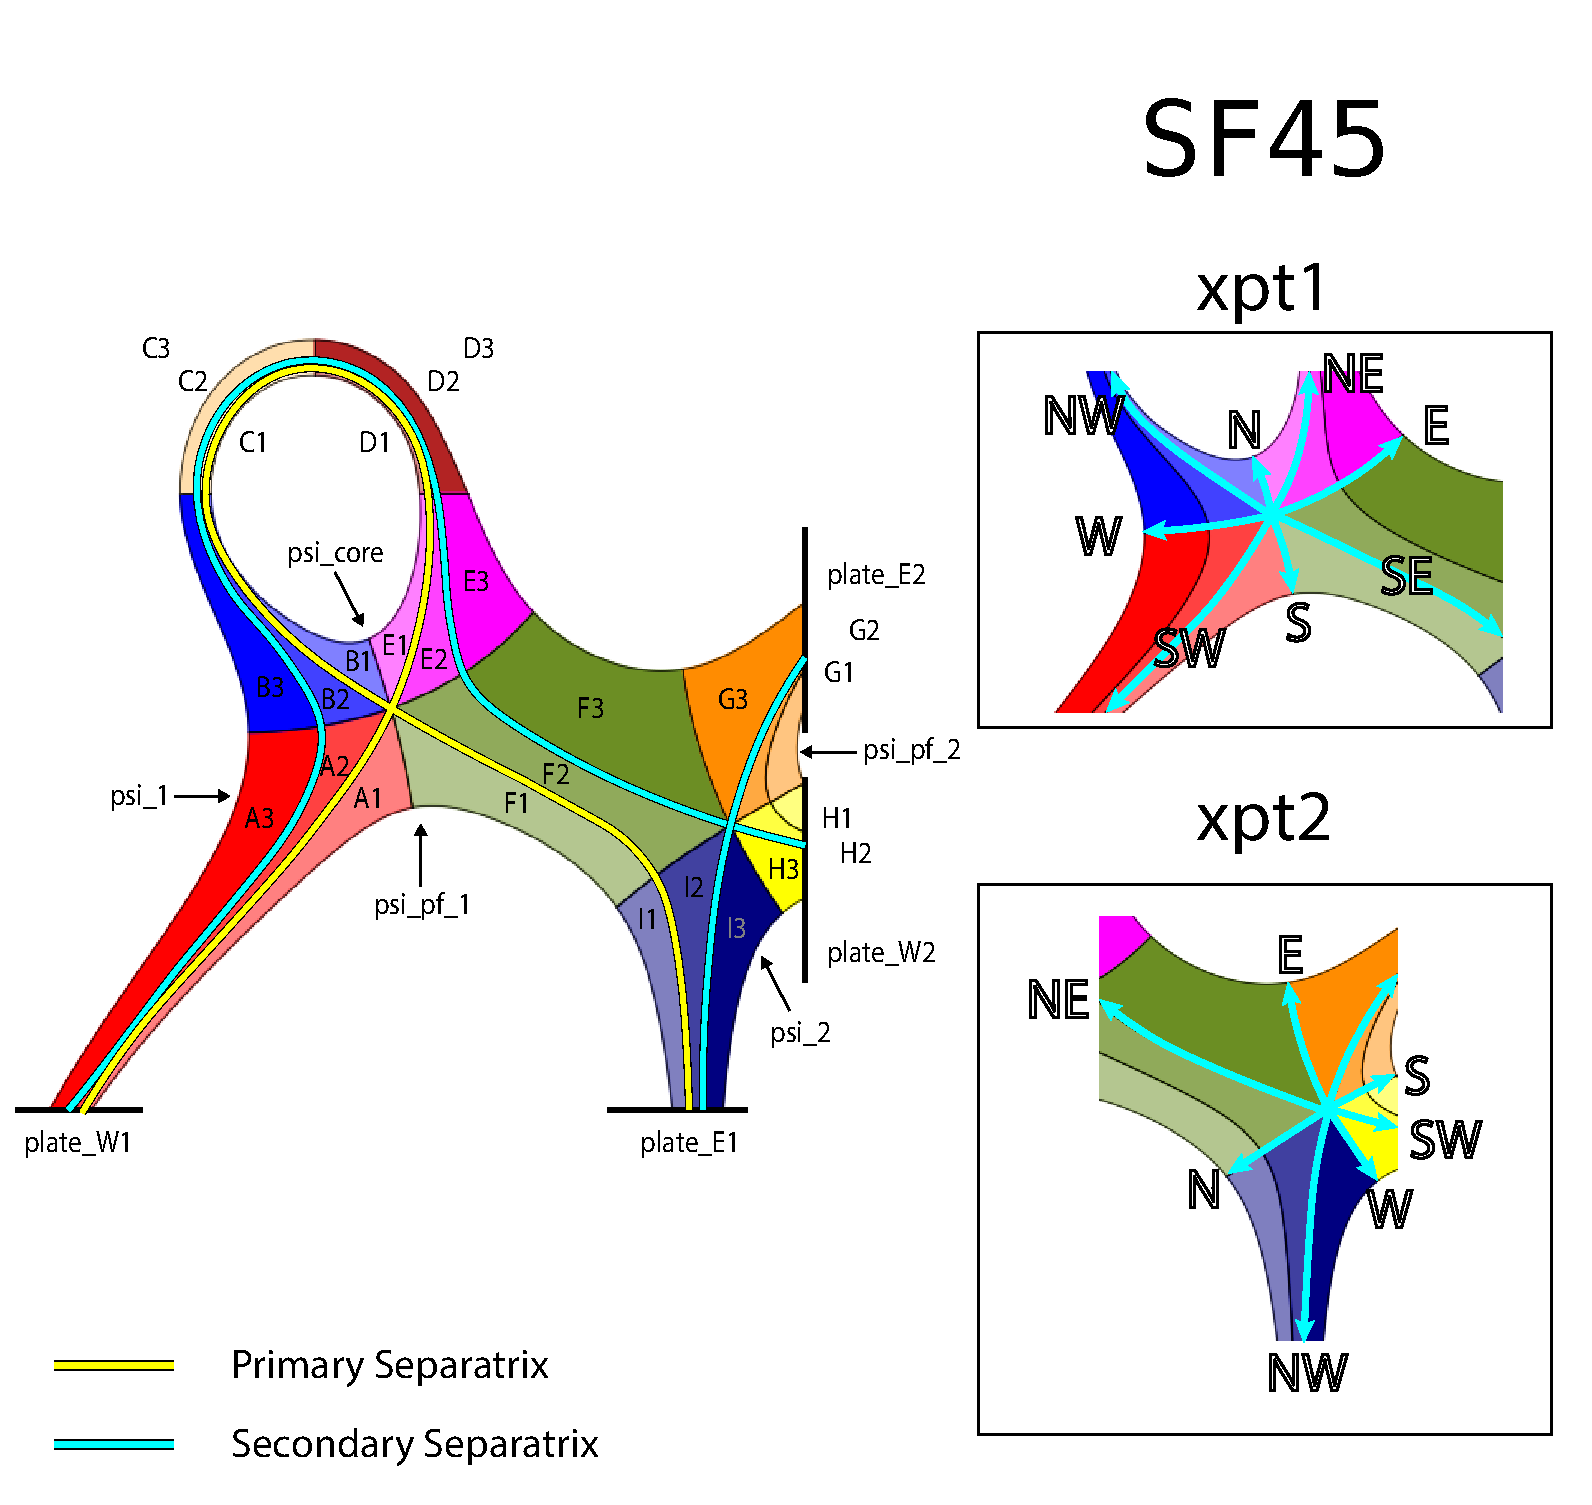
\includegraphics[width=1.05\textwidth]{figures/configurations/SF45_collection.pdf}
        \caption{SF45 Patch map}
        \label{fig:sf45_patch_map}
\end{figure}
\begin{figure}[H]
    \centering
        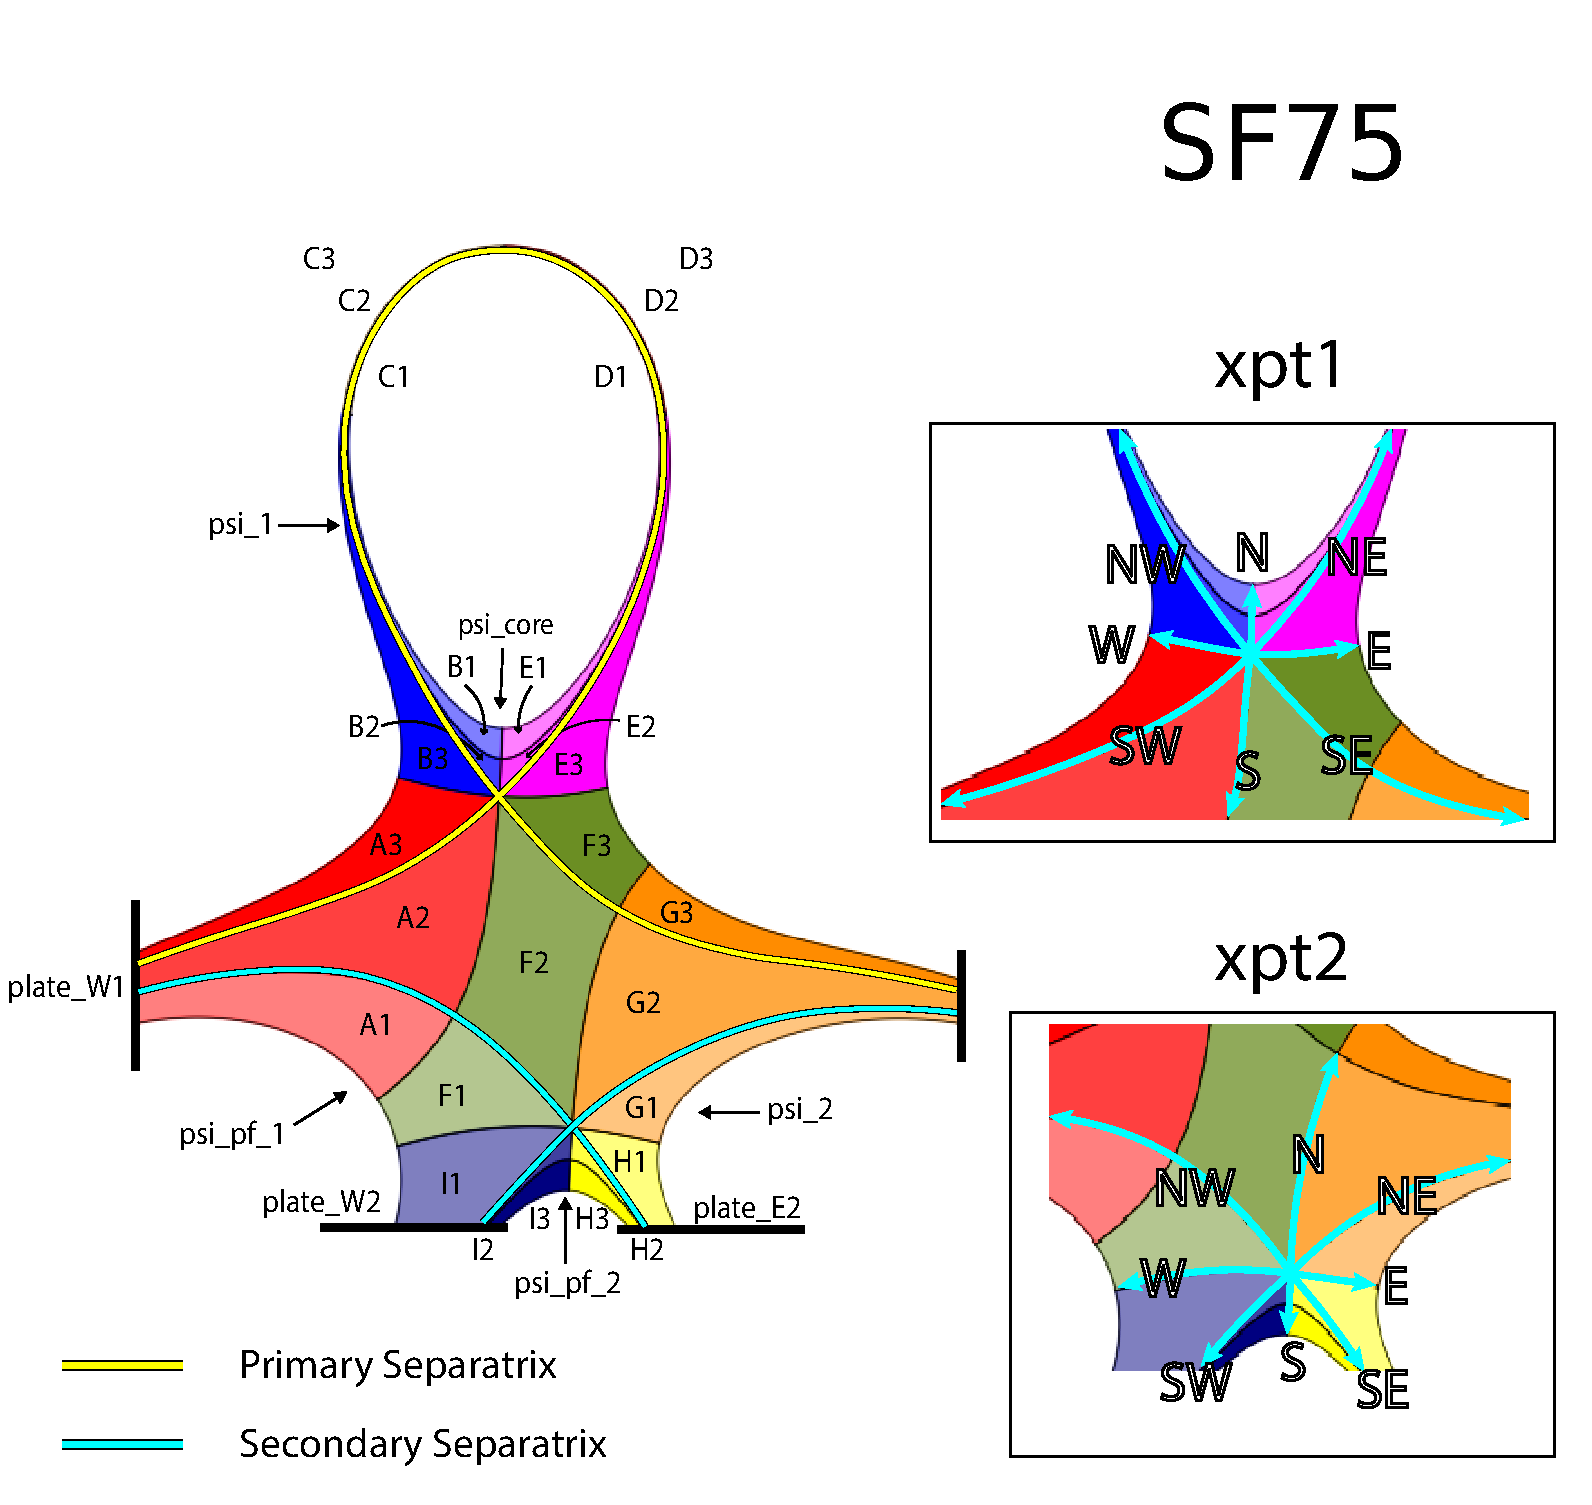
\includegraphics[width=\textwidth]{figures/configurations/SF75_collection.pdf}
        \caption{SF75 Patch map}
        \label{fig:sf75_patch_map}
\end{figure}
\begin{figure}[H]
    \centering
        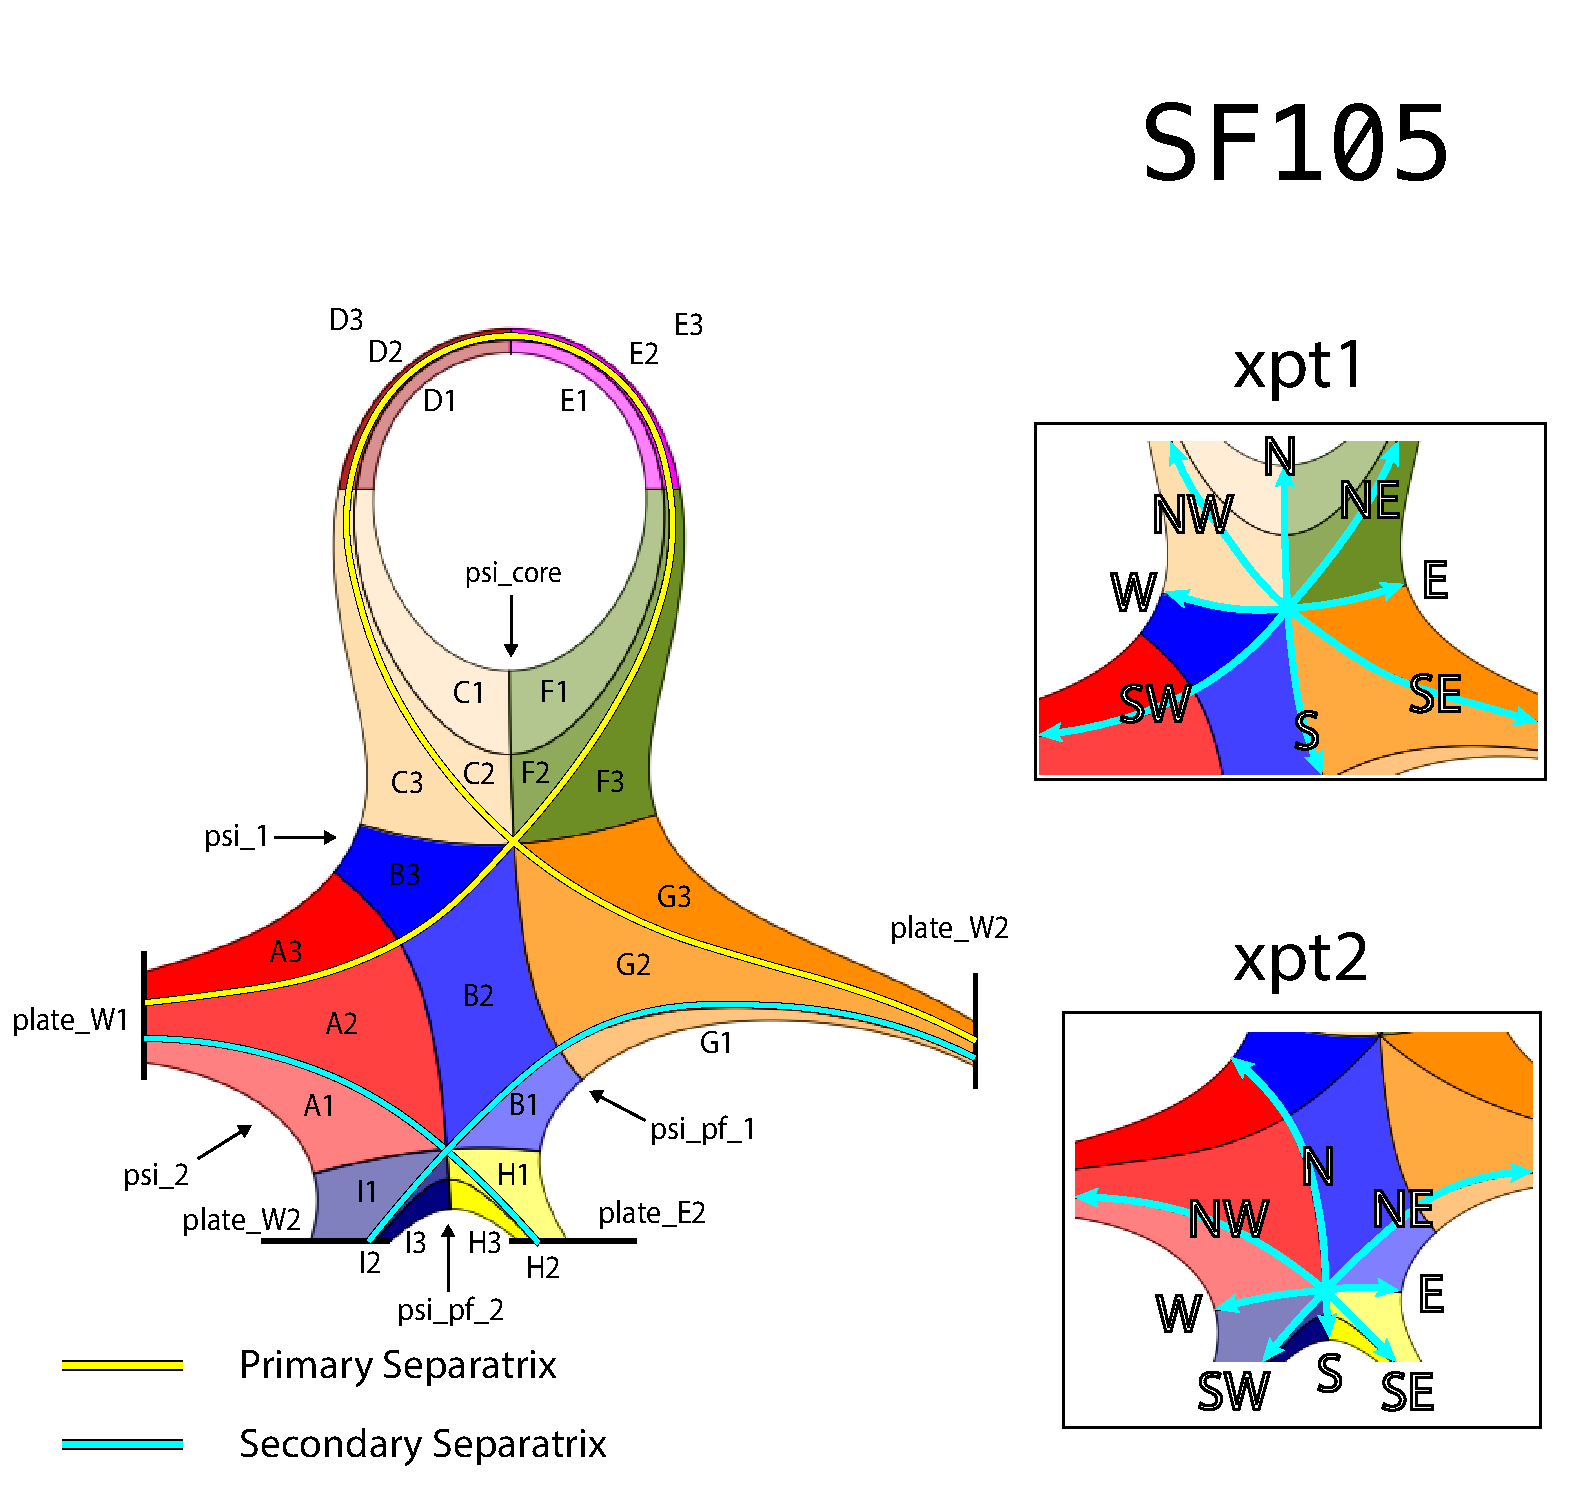
\includegraphics[width=\textwidth]{figures/configurations/SF105_collection.pdf}
        \caption{SF105 Patch map}
        \label{fig:sf105_patch_map}
\end{figure}
\begin{figure}[H]
    \centering
        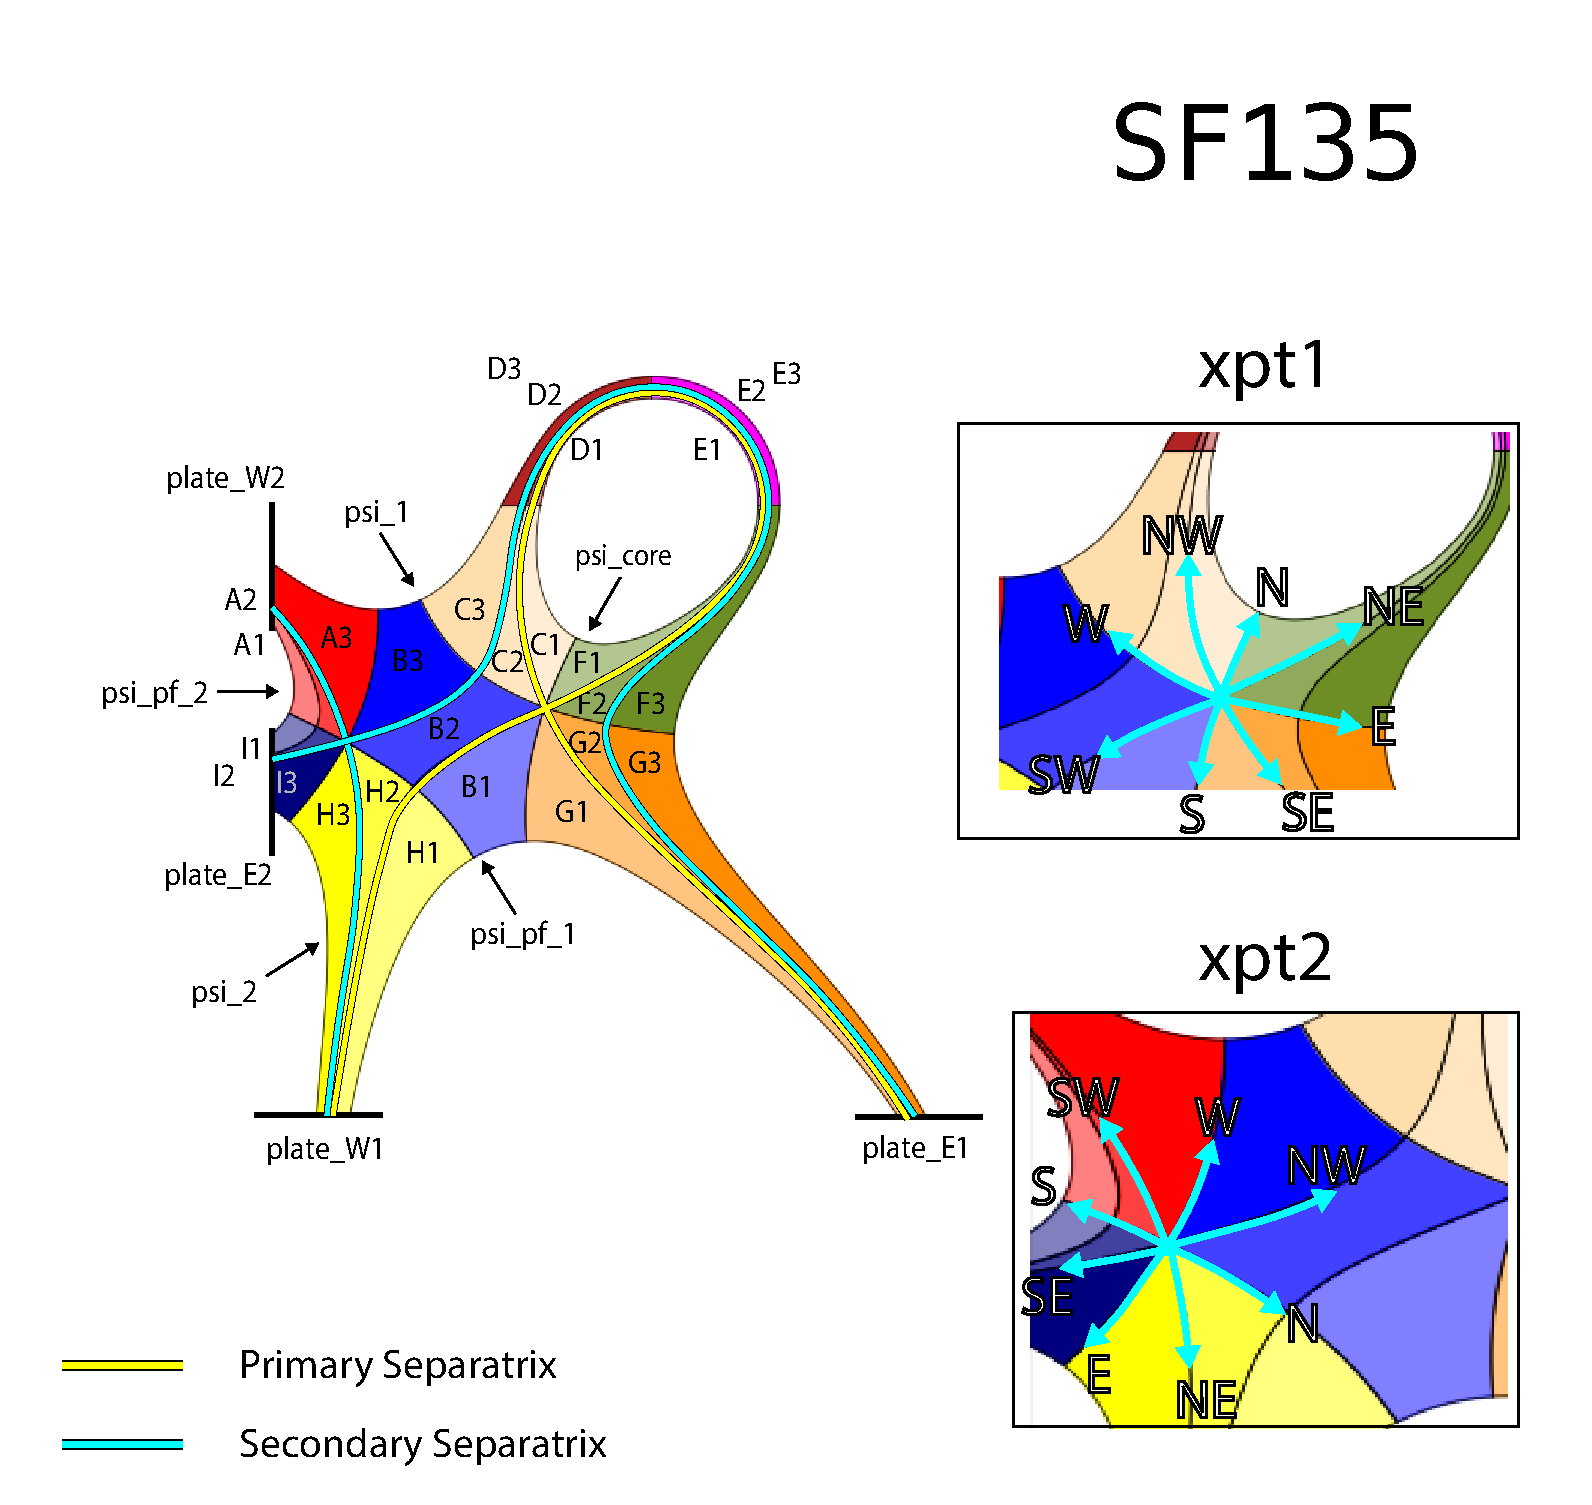
\includegraphics[width=1.05\textwidth]{figures/configurations/SF135_collection.pdf}
        \caption{SF135 Patch map}
        \label{fig:sf135_patch_map}
\end{figure}
\begin{figure}[H]
    \centering
        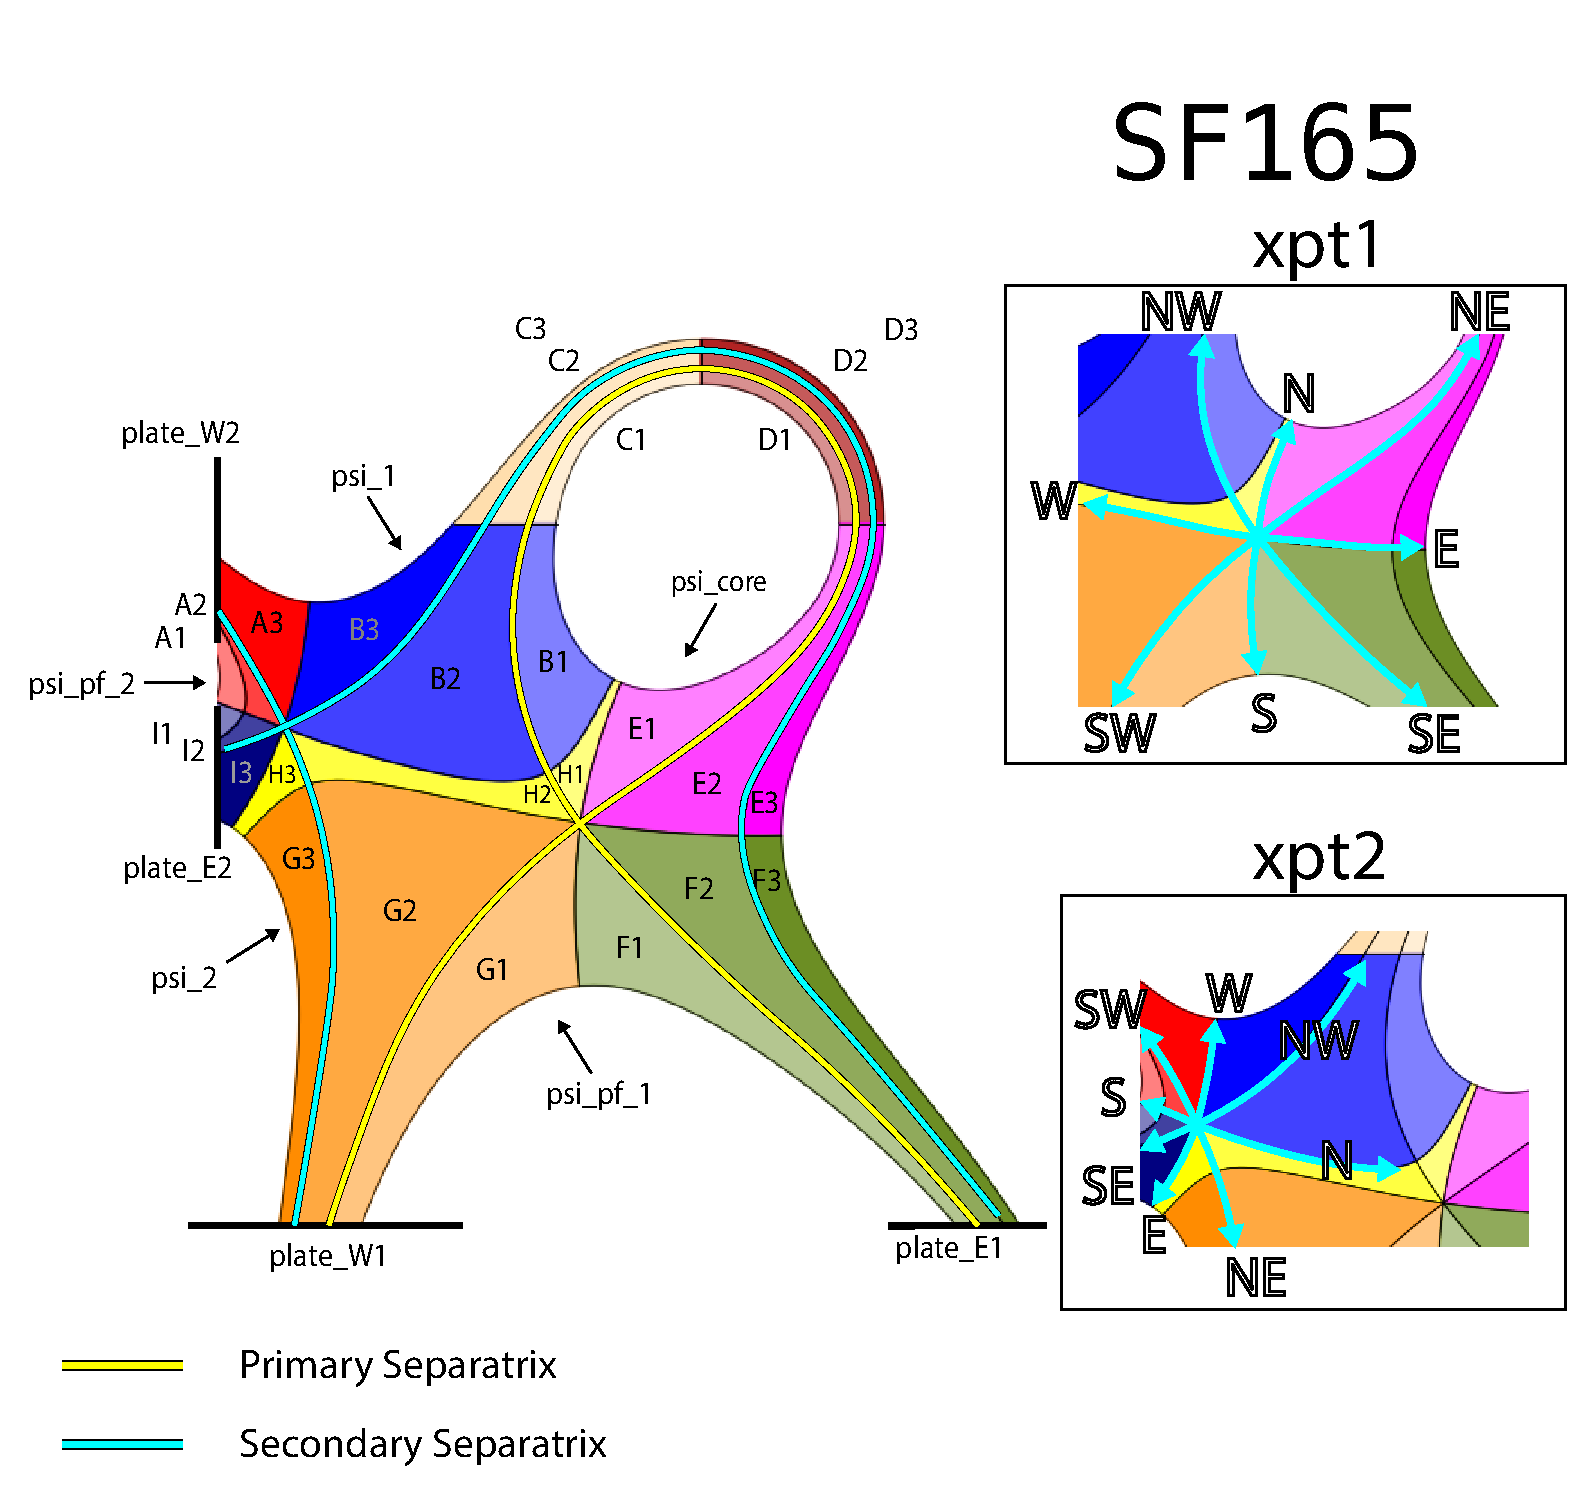
\includegraphics[width=\textwidth]{figures/configurations/SF165_collection.pdf}
        \caption{SF165 Patch map}
        \label{fig:sf165_patch_map}
\end{figure}